\chapter{Viazovska's Magic Function, Informally}

In this chapter, we will construct the $+1$-eigenfunction $a$, the $-1$-eigenfunction $b$, and the magic function $g$. The theory developed in \Cref{Ch3:Chapter} tells us what properties we would like all three functions to satisfy, and in \Cref{Ch3:Sec:Properties}, we summarised those properties concisely. Over the course of this chapter, we prove that they do, indeed, satisfy them.

We begin by defining the functions in question. In each subsequent section of this chapter, we will prove a certain property for each of the eigenfunctions. Finally, in \Cref{Ch4:Sec:g_Properties}, we will prove that $g$ does, indeed, satisfy the properties outlined in \Cref{Ch3:Chapter}.

\section{Defining Viazovska's Fourier Eigenfunctions}

The $\pm$-eigenfunctions of $g$---and, by extension, $g$ itself---are defined in terms of modular and quasimodular forms (recall the definitions of these terms from \Cref{Ch2:Sec:ModForms}). Specifically, the $+1$-eigenfunction $a$ is defined in terms of the so-called $\phi$- and $\psi$-functions, which are in turn defined in terms of the Eisenstein series (cf. \sorry) and the discriminant form (cf. \sorry), while the $-1$-eigenfunction $b$ is defined in terms of the Jacobi Theta functions (cf. \sorry)\todo{Define in Chapter 2 and cross-ref here}.

We begin by defining the $+1$-eigenfunction $a$.

\subsection{The $+1$-Eigenfunction}

We begin by defining the $\phi$-functions.

\begin{boxdefinition}[The $\phi$-Functions]\label{Ch4:Def:phis}
    Define the functions $\phi_0, \phi_{-2}, \phi_{-4} : \Halfplane \to \C$ by
    \begin{align}
        \phi_{-4} &:= \frac{E_4^2}{\Delta}
            \label{Ch4:Eq:phi_-4_def} \\
        \phi_{-2} &:= \frac{E_4\parenth{E_2 E_4 - E_6}}{\Delta}
            \label{Ch4:Eq:phi_-2_def} \\
        \phi_{0} &:= \frac{\parenth{E_2 E_4 - E_6}^2}{\Delta}
            \label{Ch4:Eq:phi_0_def}
    \end{align}
\end{boxdefinition}

These functions admit important transformation properties that are necessary to prove that the $+1$-eigenfunction is made up of integrals of holomorphic functions. This fact will in turn allow us to apply the Cauchy-Goursat Theorem (and variants thereof) that will allow us to shift contours of integration.

\begin{boxlemma}
    For all $z \in \Halfplane$,
    \begin{align}
        \phi_0\of{z + 1}
        &= \phi_0\of{z}
        \label{Ch4:Eq:phi_0_add_one} \\
        \phi_0\of{\frac{-1}{z}}
        &= \phi_0\of{z}
        - \frac{12 i}{\pi} \cdot \frac{1}{z} \cdot \phi_{-2}\of{z}
        - \frac{36}{\pi^2} \cdot \frac{1}{z^2} \cdot \phi_{-4}\of{z}
        \label{Ch4:Eq:phi_0_neg_inv}
    \end{align}
\end{boxlemma}

The proofs of these involve transformations of $E_2$, $E_4$, $E_6$, and $\Delta$, and can be found in \cite{blueprint}. We now define the $+1$-eigenfunction $a$.

\begin{boxdefinition}[Viazovska's $+1$-Fourier Eigenfunction]\label{Ch4:Def:a}
    Define $a\rad : \R \to \C$ by
    \begin{align}
        a\rad\of{r} := I_1(r) + I_2(r) + I_3(r) + I_4(r) + I_5(r) + I_6(r)
            \label{Ch4:Eq:a_rad_def}
    \end{align}
    where, for all $r \in \R$,
    \begin{align}
        I_1(r) &:= \int_{-1}^{-1 + i} \phi_0\of{\frac{-1}{z+1}} \,
                                 \parenth{z + 1}^2 \,
                                 e^{\pi i r z} \,
                                 \diff{z}
            \label{Ch4:Eq:I_1_def} \\
        I_2(r) &:= \int_{-1 + i}^{i} \phi_0\of{\frac{-1}{z+1}} \,
                                 \parenth{z + 1}^2 \,
                                 e^{\pi i r z} \,
                                 \diff{z}
            \label{Ch4:Eq:I_2_def} \\
        I_3(r) &:= \int_{1}^{1 + i} \phi_0\of{\frac{-1}{z - 1}} \,
                                \parenth{z - 1}^2 \,
                                e^{\pi i r z} \,
                                \diff{z}
            \label{Ch4:Eq:I_3_def} \\
        I_4(r) &:= \int_{1 + i}^{i} \phi_0\of{\frac{-1}{z - 1}} \,
                                \parenth{z - 1}^2 \,
                                e^{\pi i r z} \,
                                \diff{z}
            \label{Ch4:Eq:I_4_def} \\
        I_5(r) &:= -2 \int_{0}^{i} \phi_0\of{\frac{-1}{z}} \,
                                z^2 \,
                                e^{\pi i r z} \,
                                \diff{z}
            \label{Ch4:Eq:I_5_def} \\
        I_6(r) &:= 2 \int_{i}^{i \infty} \phi_0\of{z} \,
                                e^{\pi i r z} \,
                                \diff{z}
            \label{Ch4:Eq:I_6_def}
    \end{align}
    Define the $+1$-Fourier eigenfunction $a : \R^8 \to \C$ by
    \begin{align}
        a(x) := a\rad\of{\norm{x}^2}
            \label{Ch4:Eq:a_def}
    \end{align}
\end{boxdefinition}

It is immediate from \eqref{Ch4:Eq:a_def} that $a$ is radial. All of its properties are determined by its radial part $a\rad$. There are similar definitions in Lean.

There is an important remark that must be made about the definitions in \eqref{Ch4:Eq:I_1_def}-\eqref{Ch4:Eq:I_6_def}: in the original paper \cite{Viazovska8}, the integrals $I_1$ and $I_2$ are combined, as are $I_3$ and $I_4$, and expressed in the following manner:
\begin{align*}
    I_1(r) + I_2(r) &= \int_{-1}^{i} \phi_0\of{\frac{-1}{z+1}} \, \parenth{z + 1}^2 \, e^{\pi i r z} \, \diff{z} \\
    I_3(r) + I_4(r) &= \int_{1}^{i} \phi_0\of{\frac{-1}{z - 1}} \, \parenth{z - 1}^2 \, e^{\pi i r z} \, \diff{z}
\end{align*}
with the contours not specified. The most `classical' choice would be quarter-circular contours, though the same results can be achieved working with straight and rectangular contours.

\begin{figure}[ht]
    \centering
    % First subfigure: quarter-circular contour
    \begin{subfigure}{0.3\textwidth}
        \centering
        \begin{tikzpicture}[scale=1.75]
            % Axes
            \draw[->] (-1.2,0) -- (1.2,0) node[right] {$\Re$};
            \draw[->] (0,-1.2) -- (0,1.2) node[above] {$\Im$};

            % Quarter-circle from -1 to i
            \draw[thick, domain=180:135, ->] plot ({cos(\x)}, {sin(\x)}) node[above left] {$I_1 + I_2$};
            \draw[thick, domain=135:90, -] plot ({cos(\x)}, {sin(\x)}) ;

            % Points of interest
            \labelledpoint{-1}{0}{0}{-0.8}{$-1$}
            \labelledpoint{0}{1}{0.25}{-0.4}{$i$}
        \end{tikzpicture}
        \label{Ch4:subfig:a_circ_contour}
        \caption{Quarter-Circular Contour}
    \end{subfigure}
    \hfill
    % Second subfigure: straight line
    \begin{subfigure}{0.3\textwidth}
        \centering
        \begin{tikzpicture}[scale=1.75]
            % Axes
            \draw[->] (-1.2,0) -- (1.2,0) node[right] {$\Re$};
            \draw[->] (0,-1.2) -- (0,1.2) node[above] {$\Im$};

            % Straight line from -1 to 1
            \draw[thick, ->] (-1,0) -- (-0.5,0.5) node[above left] {$I_1 + I_2$};
            \draw[thick, -] (-0.5,0.5) -- (0,1);

            % Points of interest
            \labelledpoint{-1}{0}{0}{-0.8}{$-1$}
            \labelledpoint{0}{1}{0.25}{-0.4}{$i$}
        \end{tikzpicture}
        \label{Ch4:subfig:a_lin_contour}
        \caption{Straight Line Contour}
    \end{subfigure}
    \hfill
    % Third subfigure: rectangular contour
    \begin{subfigure}{0.3\textwidth}
        \centering
        \begin{tikzpicture}[scale=1.75]
            % Axes
            \draw[->] (-1.2,0) -- (1.2,0) node[right] {$\Re$};
            \draw[->] (0,-1.2) -- (0,1.2) node[above] {$\Im$};

            % Rectangular contour
            \draw[thick, ->] (-1,0) -- (-1,0.5) node[left] {$I_1$};
            \draw[thick, -] (-1,0.5) -- (-1,1);
            \draw[thick, ->] (-1,1) -- (-0.5,1) node[above] {$I_2$};m
            \draw[thick, -] (-0.5,1) -- (0,1);

            % Points of interest
            \labelledpoint{-1}{0}{0}{-0.8}{$-1$}
            \labelledpoint{0}{1}{0.25}{-0.4}{$i$}
            \labelledpoint{-1}{1}{-0.7}{-0.2}{$-1 + i$}
        \end{tikzpicture}
        \label{Ch4:subfig:a_rect_contour}
        \caption{Rectangular Contour}
    \end{subfigure}
    \caption{\centering Different contours along which we can integrate the integrand of $I_1$ and $I_2$ to get an integral equal to $I_1 + I_2$}
    \label{Ch4:fig:a_contours}
\end{figure}

The reason the choice of contours does not matter is that in the integrands of $I_1, \ldots, I_5$, we multiply terms of the form $\phi_0\of{\frac{-1}{z}}$ by $z^2$. If we apply \eqref{Ch4:Eq:phi_0_neg_inv} and multiply through, it is clear that we are removing any singularities introduced by $\frac{1}{z^2}$ and $\frac{1}{z}$ factors. We can then use the fact that $\Delta\of{z} \neq 0$ for all $z \in \Halfplane$ to conclude that the integrands are holomorphic up to these removable singularities.

The choice of rectangular contours (as in \Cref{Ch4:subfig:a_rect_contour}) as opposed to quarter-circles or straight lines for $I_1 + I_2$ and $I_3 + I_4$ is motivated by the versions of the Cauchy-Goursat Theorem that have been formalised in Lean.

% Insert a visual here for I_1, and say I_2 is analogous

We are now ready to define the $-1$-eigenfunction $b$.

\subsection{The $-1$-Eigenfunction}

Recall the definitions of the $H$-functions defined in \sorry\ to be the fourth powers of the thetanullwerte. We begin by defining the $h$ function, in terms of which we will define the $\psi$-functions.

\begin{boxdefinition}[The $h$-Function]\label{Ch4:Def:h}
    Define the function $h : \Halfplane \to \C$ by
    \begin{align}
        h\of{z} := 128 \frac{H_3(z) + H_4(z)}{H_2(z)^2} \label{Ch4:Eq:h_def}
    \end{align}
    where $H_2, H_3, H_4$ are as defined in \sorry.
\end{boxdefinition}

In \cite{Viazovska8}, the $\psi$-functions are defined in terms of the $h$-function via slash actions. We express them in terms of $h$ more directly.

\begin{boxdefinition}[The $\psi$-Functions]\label{Ch4:Def:psis}
    Define the functions $\psi_I, \psi_S, \psi_T : \Halfplane \to \C$ by
    \begin{align}
        \psi_I\of{z} &:= h\of{z}^3
            \label{Ch4:Eq:psi_I_def} \\
        \psi_S\of{z} &:= -h\of{z}^3
            \label{Ch4:Eq:psi_S_def} \\
        \psi_T\of{z} &:= h\of{z}^3 - h\of{z}^3
            \label{Ch4:Eq:psi_T_def}
    \end{align}
    where $h$ is as defined in \Cref{Ch4:Def:h}.
\end{boxdefinition}

\begin{boxproposition}[The $\psi$-Fucntions]\label{Ch4:Prop:psi_as_div_disc}
    We can express $\psi_I, \psi_S, \psi_T$ in the following manner:
    \begin{align}
        \psi_I &= \frac{H_4^3\parenth{2 H_4^2 + 5 H_4 H_2 + 5 H_2^2}}{2 \Delta}
            \label{Ch4:Eq:psi_I_def} \\
        \psi_S &= \frac{- H_2^3 \parenth{2 H_2^3 + 5 H_2 H_4 + 5 H_4^2}}{2 \Delta}
            \label{Ch4:Eq:psi_S_def} \\
        \psi_T &= \psi_I - \psi_S
            \label{Ch4:Eq:psi_T_def}
    \end{align}
    where $\Delta$ is the discriminant form.
\end{boxproposition}
\section{Establishing the Schwartzness Property}

The magic function is a linear combination of $a$ and $b$, which are each defined as compositions of $a\rad$ and $b\rad$ with the norm-squared function. From \Cref{Ch3:Prop:Multidimensional_Schwartz_of_Schwartz}, we know that it is enough to establish that $a\rad$ and $b\rad$ are Schwartz to establish that $a$ and $b$ are Schwartz. In particular, this means the smoothness and decaying conditions need to be satisfied with respect to $\R$ inputs instead of $\R^8$ inputs, a substantial simplification. We can further simplify the problem by taking advantage of linearity.

We know that the Schwartz space is a $\C$-vector space, making it closed under addition. To show that $a\rad$ and $b\rad$ are Schwartz functions, we show that their constituent integrals $I_1, \ldots, I_6$ and $J_1, \ldots, J_6$ are Schwartz. We need to show both smoothness and rapid decay. Smoothness is fairly straightforward. Rapid decay, on the other hand, requires an additional ingredient.

It turns out that we can establish a general result that yields an upper-bound for functions of the form $\frac{f}{\Delta}$, where $\Delta$ is the discriminant form and there is a polynomial growth condition on the Fourier coefficients of $f$. We take advantage of the fact that the $\phi$- and $\psi$-functions can be expressed in this form (cf. \Cref{Ch4:Def:phis} and \Cref{Ch4:Prop:psi_as_div_disc}). The condition on their Fourier coefficients comes from the theory of modular forms.

We begin with the statement and proof of the general result \cite[Lemma 7.4]{blueprint}.\todo{UPDATE LEMMA NUMBER BEFORE SUBMITTING}

\begin{boxtheorem}\label{SP:PolyFourierCoeffBound}
    Let $f : \C \to \C$ be holomorphic. Denote by $c_f(n)$ its $n$th Fourier coefficient, with $c_f\of{n_0} \neq 0$, so that
    \begin{align*}
        f(z) = \sum_{n=n_0}^{\infty} c_f(n) \, e^{i \pi n z}
    \end{align*}
    If there exists $k \in \N$ such that $c_f(n) = \BigO{n^k}$ as $n \to \infty$, then there exists a constant $C_f > 0$ such that for all $z \in \Halfplane$ with $\Im\of{z} > 1/2$,
    \begin{align*}
        \abs{\frac{f(z)}{\Delta(z)}} \leq C_f \, e^{-\pi \parenth{n_0 - 2} \Im(z)}
    \end{align*}
\end{boxtheorem}
\begin{proof}
    Fix $z \in \Halfplane$ and assume $\Im(z) > 1/2$. Recall from \Cref{Ch2:Thm:Delta_Product_Formula} that $\Delta$ can be expressed as a (convergent) infinite product. We can hence write
    \begin{align*}
        \abs{\frac{f(z)}{\Delta(z)}}
        = \abs{\frac{\sum_{n = n_0}^{\infty} c_f(n) \, e^{\pi i n z}}{e^{2 \pi i z} \prod_{n=1}^{\infty} \parenth{1 - e^{2 \pi i n z}}^{24}}}
        = \abs{e^{\pi i \parenth{n_0 - 2} z}} \cdot \frac{\abs{\sum_{n=n_0}^{\infty} c_f(n) \, e^{\pi i \parenth{n - n_0} z}}}{\prod_{n=1}^{\infty} \abs{1 - e^{2 \pi i n z}}^{24}}
    \end{align*}
    Noting that $\abs{e^{iz}} = e^{-\Im(z)}$ and $\Im(z) > \frac{1}{2}$, we can see that
    \begin{align*}
        \abs{e^{\pi i \parenth{n_0 - 2} z}} \cdot \frac{\abs{\sum_{n=n_0}^{\infty} c_f(n) \, e^{\pi i \parenth{n - n_0} z}}}{\abs{\prod_{n=1}^{\infty} {1 - e^{2 \pi i n z}}^{24}}}
        \leq
        e^{-\pi \parenth{n - n_0} \Im(z)} \cdot \frac{\sum_{n=0}^{\infty} \abs{c_f(n)} \, e^{-\pi \parenth{n - n_0}/2}}{\abs{\prod_{n=1}^{\infty} {1 - e^{2 \pi i n z}}^{24}}}
    \end{align*}
    It has been \href{https://github.com/leanprover-community/mathlib4/blob/5a2eaa85c555c4263e15928cef249cbaad2eb2d2/Mathlib/Topology/Algebra/InfiniteSum/Order.lean#L379-L380}{verified formally} that the absolute value of a convergent infinite product is the product of the absolute values, and moreover, that the product of the absolute values is \href{https://github.com/leanprover-community/mathlib4/blob/5a2eaa85c555c4263e15928cef249cbaad2eb2d2/Mathlib/Topology/Algebra/InfiniteSum/Order.lean#L373-L374}{convergent}. It has also been \href{https://github.com/thefundamentaltheor3m/Sphere-Packing-Lean/blob/ba092be9cdebb1a9c170a22c234e71ca1842a173/SpherePacking/ForMathlib/tprod.lean#L28}{verified formally} that the infinite product is monotonic on convergent infinite products whose terms are nonnegative. Hence,
    \begin{align*}
        \abs{\prod_{n=1}^{\infty} \parenth{1 - e^{2 \pi i n z}}^{24}}
        = \prod_{n=1}^{\infty} \abs{1 - e^{2 \pi i n z}}^{24}
        \geq \prod_{n=1}^{\infty} \parenth{1 - e^{-2 \pi n \Im(z)}}^{24}
        \geq \prod_{n=1}^{\infty}\parenth{1 - e^{-\pi n}}^{24}
    \end{align*}
    We note that the third and fourth products are convergent because they are expressible, via the product formula, as $e^{2\pi\Im(z)} \Delta\of{i \cdot \Im(z)}$ and $e^{\pi} \Delta\of{i/2}$ respectively. Hence, defining
    \begin{align*}
        C_f := \frac{\sum_{n=0}^{\infty} \abs{c_f(n)} \, e^{-\pi \parenth{n - n_0}/2}}{\prod_{n=1}^{\infty}\parenth{1 - e^{-\pi n}}^{24}}
    \end{align*}
    we can see that $\abs{\frac{f(z)}{\Delta(z)}} \leq C_f \, e^{-\pi \parenth{n_0 - 2} \Im(z)}$, as desired.
\end{proof}

A key step in showing that $a\rad$ and $b\rad$ are Schwartz will be to bound the $\phi$- and $\psi$-functions using \Cref{SP:PolyFourierCoeffBound}. Since these functions are defined as sums and products of the Eisenstein series and the $H$-functions, whose Fourier coefficients have polynomial growth (as seen in \Cref{Ch2:Sec:ModForms}) and admit indices $n_0$ below which all Fourier coefficients are zero, it is enough to show that sums and products of functions that exhibit this property inherit it. This is clear for sums, and we omit the proof, but we prove it explicitly for products.

\begin{boxproposition}
    Let $f_1, f_2 : \Halfplane \to \C$ be functions with (absolutely convergent) Fourier expansions
    \begin{align*}
        f_1(z) &= \sum_{n=n_1}^{\infty} c_1(n) \, e^{\pi i n z} \\
        f_2(z) &= \sum_{n=n_2}^{\infty} c_2(n) \, e^{\pi i n z}
    \end{align*}
    such that for $i \in \set{1, 2}$, $c_i(n_i) \neq 0$ and $\exists k_i \in \N$ such that $c_i(n) = \BigO{n^{k_i}}$ as $n \to \infty$. Then, their product $f_1 f_2$ is expressible as an absolutely convergent Fourier series
    \begin{align*}
        f_1(z) f_2(z) &= \sum_{n = n_0}^{\infty} c(n) \, e^{\pi i n z}
    \end{align*}
    such that $c(n_0) \neq 0$ and $\exists k \in \N$ such that $c(n) = \BigO{n^k}$ as $n \to \infty$.
\end{boxproposition}
\begin{proof}
    Fix $z \in \Halfplane$. Then, due to absolute convergence, we can write
    \begin{align*}
        f_1(z) f_2(z) &= \parenth{\sum_{n=n_1}^{\infty} c_1(n) \, e^{\pi i n z}} \parenth{\sum_{m=n_2}^{\infty} c_2(m) \, e^{\pi i m z}} \\
        &= \sum_{n = n_1}^{\infty} \sum_{m = n_2}^{\infty} c_1(n) c_2(m) \, e^{\pi i \parenth{n + m} z}
    \end{align*}
    The smallest value of $m + n$ is clearly $n_1 + n_2$, so we can take this to be $n_0$. So, we can write
    \begin{align*}
        f_1(z) f_2(z) &= \sum_{\ell = n_0}^{\infty} c(n) \, e^{\pi i \ell z}
    \end{align*}
    where for each $\ell \geq n_0$, $c(\ell)$ is a sum of finitely many terms of the form $c_1(n) c_2(m)$, with $n + m = \ell$. Now, we know $\exists C, D \in \R$ and $N, M \in \N$ such that for all $n \geq N$ and $m \geq M$, $\abs{c_1(n)} \leq C \abs{n^{k_1}}$ and $\abs{c_2(m)} \leq D \abs{m^{k_2}}$. Then, \sorry
\end{proof}

We now show that $a\rad$, the radial version of the $+1$-eigenfunction, is Schwartz.

\subsection{The $+1$-Eigenfunction}

We begin by proving that $I_1, \ldots, I_6$ are smooth. The key to proving this is the Leibniz Integral Rule\footnote{Also known as Leibniz's technique for `differentiating under the integral sign'}, which states that under mild conditions, the derivative with respect to one variable of the integral with respect to the other variable of a function of two variables is given by the integral of the corresponding partial derivative, which implies the analogous differentiability criterion.

\begin{boxlemma}
    For all $1 \leq j \leq 6$ and $k \in \N$, $I_j(r)$ is $k$ times differentiable.
\end{boxlemma}
\begin{proof}
    Fix $1 \leq j \leq 6$. We know, from \Cref{Ch4:Def:a}, that
    \begin{align*}
        I_j(r) = \int_{X_j} g_j\of{z} \, e^{\pi i r z} \, \diff{z}
    \end{align*}
    for intervals $X_j$ and holomorphic functions $g_j : \Halfplane \to \C$. The Leibniz Integral Rule then tells us that for all $k \in \N$, the $k$th derivative of $I_j$ at some $r \in \R$ is given by
    \begin{align}
        \int_{X_j} g_j\of{z} \, \parenth{\pi i z}^{k} \, e^{\pi i r z} \, \diff{z}
        \label{Ch4:Eq:Ij_deriv}
    \end{align}
    In particular, $I_j$ is smooth (in $r$) for all $j$.
\end{proof}

We are now ready to prove that $I_1, \ldots, I_6$ and their derivatives satisfy the decaying property. As a first step, we show that we can apply \Cref{SP:PolyFourierCoeffBound}.

\begin{boxlemma}\label{Ch4:Lemma:PolyFourierCoeffBound_Apply}
    There exist real numbers $C_0, C_{-2}, C_{-4} > 0$ such that
    \begin{align*}
        \abs{\phi_0\of{z}} &\leq C_{0} e^{-2\pi\Im(z)} \\
        \abs{\phi_{-2}\of{z}} &\leq C_{-2} \\
        \abs{\phi_{-4}\of{z}} &\leq C_{-4} e^{2\pi\Im(z)}
    \end{align*}
    for all $z \in \Halfplane$ with $\Im(z) > \frac{1}{2}$.
\end{boxlemma}
\begin{proof}
    Fix $z \in \Halfplane$ and assume that $\Im(z) > \frac{1}{2}$. The following is a consequence of a result proved by Ramanujan \todo{find citation for original paper} in the theory of (quasi-)modular forms:
    \begin{align}
        E_2 E_4 - E_6 &= 720 \sum_{n=1}^{\infty} n \, \sigma_3(n) \, e^{2\pi i nz}
        \label{Ch4:Eq:E2E4_sub_E6_qexpansion}
    \end{align}
    with the sum converging absolutely. Furthermore, it is easily seen that $\sigma_3(n) = \BigO{n^4}$, since $\sigma_3(n)$ is the sum of at most $n$ elements that are each at most $n^3$. Then, combining \eqref{Ch4:Eq:E2E4_sub_E6_qexpansion} and \eqref{Ch2:Eq:E4_qexpansion}, one can show that $E_4^2$, $E_4\parenth{E_2 E_4 - E_6}$, and $\parenth{E_2 E_4 - E_6}$ all have Fourier expansions in which each Fourier coefficient is $\BigO{n^{10}}$. For instance, we know
    \begin{align}
        \parenth{E_2 E_4 - E_6}^2 = 720^2 \sum_{m=1}^{\infty} \sum_{n=1}^{\infty} n \, \sigma_3(n) \, e^{2\pi i z \parenth{m + n}}
        \label{Ch4:Eq:E2E4_sub_E6_sq_qexpansion}
    \end{align}
    The Fourier coefficient corresponding to a term of the form $e^{2 \pi i z \parenth{m + n}}$ is a sum of at most $m + n$ terms that are each bounded above by $\parenth{\parenth{m + n}\sigma_3\of{m + n}}^2$, which is $\BigO{\parenth{m + n}^{10}}$. Similar computations can be performed for $E_4^2$ and $E_4\parenth{E_2 E_4 - E_6}$, proving that the polynomial growth assumption of \Cref{SP:PolyFourierCoeffBound} is satisfied by $\phi_{-4}$, $\phi_{-2}$ and $\phi_0$.

    We also note from \eqref{Ch4:Eq:E2E4_sub_E6_sq_qexpansion} that the smallest nonzero Fourier coefficient corresponds to $m + n = 2$. Reconciling this with the fact that in the statement of \Cref{SP:PolyFourierCoeffBound}, we express the Fourier series in terms of powers of $e^{\pi i z}$ and not $e^{2 \pi i z}$, we conclude that the right choice of $n_0$ to bound $\phi_0$ is $4$. Similar computations show that the right value for $\phi_{-2}$ is $2$ and that for $\phi_{-4}$ is $0$, which allows us to apply \Cref{SP:PolyFourierCoeffBound} and conclude that there exist $C_0, C_{-2}, C_{-4} > 0$ such that
    \begin{align*}
        \abs{\phi_0\of{z}} &\leq C_{0} e^{-2\pi\Im(z)} \\
        \abs{\phi_{-2}\of{z}} &\leq C_{-2} \\
        \abs{\phi_{-4}\of{z}} &\leq C_{-4} e^{2\pi\Im(z)}
    \end{align*}
    as required.
\end{proof}

We can now bound $I_1$, $I_3$ and $I_5$.

\begin{boxlemma}\label{Ch4:Lemma:Bound_I1_I3_I5}
    There exists a positive real number $C_0$ such that for all $r \in \R$,
    \begin{align*}
        \abs{I_1(r)}, \abs{I_3(r)}, \abs{I_5(r)} &\leq \int_{1}^{\infty} C_0 \, e^{-2\pi s} \, e^{-\pi r/s} \, \diff{s}
    \end{align*}
\end{boxlemma}
\begin{proof}
    For conciseness, we only bound $\abs{I_1}$ explicitly. Parametrise $z = -1 + it$ in \eqref{Ch4:Eq:I_1_def}. Then, for all $r \in \R$, we can write
    \begin{align*}
        I_1(r) &= -i \int_{0}^{1}
            \phi_0\of{\frac{-1}{it}} \,
            t^2 \,
            e^{-\pi i r} \,
            e^{\pi r t}\,
            \diff{t}
    \end{align*}
    Writing $s = \frac{1}{t}$ and simplifying, we get that
    \begin{align*}
        I_1(r) &= -i \int_{1}^{\infty}
            \phi_0\of{is} \,
            s^{-4} \,
            e^{-\pi i r} \,
            e^{-\pi r / s}\,
            \diff{t}
    \end{align*}
    Applying the triangle inequality, multiplicativity and monotonicity, we get
    \begin{align*}
        \abs{I_1(r)} &\leq \int_{1}^{\infty} \abs{
            \phi_0\of{is} \,
            s^{-4} \,
            e^{-\pi i r} \,
            e^{-\pi r / s}\,
            } \diff{t}
        \leq \int_{1}^{\infty}
            \abs{\phi_0\of{is}} \,
            e^{-\pi i r/s}
    \end{align*}
    Since $s > \frac{1}{2}$ inside the integral, we know from \Cref{Ch4:Lemma:PolyFourierCoeffBound_Apply} that $\exists C_0 > 0$ such that
    \begin{align*}
        \abs{I_1(r)} \leq \int_{1}^{\infty} C_0 \, e^{-2\pi s} \, e^{-\pi r/s} \, \diff{s}
    \end{align*}
    as required. The bounds on $\abs{I_3}$ and $\abs{I_5}$ are computed similarly.
\end{proof}

Now that we have bounds on the integrals with bounded vertical contours, we compute bounds on the integrals with bounded horizontal contours.

\begin{boxlemma}\label{Ch4:Lemma:Bound_I2_I4}
    There exists a positive real number $C_1$ such that for all $r \in \R$,
    \begin{align*}
        \abs{I_2(r)}, \abs{I_4(r)} &\leq C_1 \, e^{-\pi r}
    \end{align*}
\end{boxlemma}
\begin{proof}
    For conciseness, we only bound $\abs{I_2}$ explicitly. Parametrise $z = -1 + t + i$ in \eqref{Ch4:Eq:I_2_def}. Then, for all $r \in \R$, we can write
    \begin{align*}
        I_2(r) = \int_{0}^{1}
            \phi_0\of{\frac{-1}{t + i}} \,
            \parenth{t + i}^2 \,
            e^{-\pi i r} \,
            e^{\pi i r t} \,
            e^{-\pi r} \,
            \diff{t}
    \end{align*}
    Applying the triangle inequality, multiplicativity and monotonicity, we get
    \begin{align*}
        \abs{I_2(r)} &\leq \int_{0}^{1} \abs{\phi_0\of{\frac{-1}{t + i}}} \cdot 2e^{-\pi r} \, dt
    \end{align*}
    It is therefore enough to show that \Cref{SP:PolyFourierCoeffBound} applies. To that end, we manipulate the expression inside $\phi_0$:
    \begin{align*}
        \frac{-1}{t + i} = \frac{t}{t^2 + 1} + \frac{1}{t^2 + 1}i
    \end{align*}
    From this, we can deduce that its imaginary part is greater than $\frac{1}{2}$ for all $t \in \parenth{0, 1}$. Then, \Cref{SP:PolyFourierCoeffBound} tells us that $\exists C_0 > 0$ such that
    \begin{align*}
        \abs{\phi_0\of{\frac{-1}{t + i}}}
        \leq C_0 \, e^{-2 \pi \cdot \frac{1}{t^2 + 1}}
        \leq C_0 \, e^{-2\pi \cdot \frac{1}{2}} = C_0 \, e^{-\pi}
    \end{align*}
    Then, taking $C_1 := 2 \, C_0 \, e^{-\pi}$ and applying monotonicity,
    \begin{align*}
        \abs{I_2(r)} \leq \int_{0}^{1} C_1 \, e^{-\pi r} \, \diff{t} = C_1 \, e^{-\pi r}
    \end{align*}
    as required. The bound on $\abs{I_4}$ is computed similarly.
\end{proof}

Finally, we bound the integral with the unbounded vertical contour.

\begin{boxlemma}\label{Ch4:Lemma:Bound_I6}
    There exists a positive real number $C_2$ such that for all $r \in \R$,
    \begin{align*}
        \abs{I_6(r)} &\leq C_2 \, \frac{e^{-\pi \parenth{r + 2}}}{r + 2}
    \end{align*}
\end{boxlemma}
\begin{proof}
    Parametrise $z = it$ in \eqref{Ch4:Eq:I_6_def}. Then, for all $r \in \R$, we can write
    \begin{align*}
        I_6(r) &= -2i \int_{1}^{\infty} \phi_0\of{it} \, e^{- \pi r t} \, \diff{t}
    \end{align*}
    Applying the triangle inequality, multiplicativity and monotonicity, we get
    \begin{align*}
        \abs{I_6(r)} \leq 2\int_{1}^{\infty}
            \abs{\phi_0\of{it}} \,
            e^{-\pi r t} \,
            \diff{t}
    \end{align*}
    Let $C_0$ be as in \Cref{SP:PolyFourierCoeffBound} and define $C_1 := 2 C_0$. Then,
    \begin{align*}
        \abs{I_6(r)} \leq 2\int_{1}^{\infty}
            C_0 \,
            e^{-2 \pi t} \,
            e^{-\pi r t} \,
            \diff{t}
        = C_1 \int_{1}^{\infty} e^{-\parenth{2\pi + \pi r}t} \, \diff{t}
        = C_1 \frac{e^{-\pi\parenth{r + 2}}}{\pi\parenth{r + 2}}
    \end{align*}
    Defining $C_2 := \frac{C_1}{\pi}$ then yields the desired result.
\end{proof}

The formal proofs of the bounds in \Cref{Ch4:Lemma:Bound_I1_I3_I5,Ch4:Lemma:Bound_I2_I4,Ch4:Lemma:Bound_I6} are complete up to proofs that they are bounded by integrable functions, which is necessary to apply monotonicity of the integral due to the definition of the integral in \mathlib. The evaluation of the final integral in \Cref{Ch4:Lemma:Bound_I6} is also currently a \sorry.\todo{Update}

We now demonstrate how bounds on higher derivatives of $I_1$ can be reduced to the case we saw in \Cref{Ch4:Lemma:Bound_I1_I3_I5}.

\begin{boxlemma}
    For all $k \in \N$, there exists a positive real number $C_0^{(k)}$ such that for all $r \in \R$,
    \begin{align*}
        \abs{I_1^{(k)}\of{r}} \leq \int_{1}^{\infty} C_0^{(k)} \, e^{-2\pi s} \, e^{- \pi r / s} \, \diff{s}
    \end{align*}
\end{boxlemma}
\begin{proof}
    Fix $k \in \N$ and $r \in \R$. As we showed in \eqref{Ch4:Eq:Ij_deriv}, the $k$th derivative of $I_1$ at $r$ can be expressed as
    \begin{align*}
        I_1^{(k)}\of{r} = \int_{-1}^{-1+i} \phi_0\of{\frac{-1}{z+1}} \, \parenth{z+1}^2 \, \parenth{\pi i z}^k \, e^{\pi i r z} \, \diff{z}
    \end{align*}
    Parametrise $z = -1 + it$. Then,
    \begin{align*}
        I_1^{(k)}\of{r} = -i \int_{0}^{1} \phi_0\of{\frac{-1}{it}} \, t^2 \, \parenth{-\pi i - \pi t}^k \, e^{-\pi i r} \, e^{\pi r t} \, \diff{z}
    \end{align*}
    Writing $s = \frac{1}{t}$ and simplifying, we get that
    \begin{align*}
        I_1^{(k)}\of{r} &= -i \int_{1}^{\infty}
            \phi_0\of{is} \,
            s^{-4} \,
            \parenth{-\pi i - \frac{\pi}{s}}^k \,
            e^{-\pi i r} \,
            e^{-\pi r / s}\,
            \diff{t}
    \end{align*}
    Observe that for all $s \in \Ico{1, \infty}$,
    \begin{align*}
        \abs{-\pi i - \frac{\pi}{s}} = \pi \abs{i + \frac{1}{s}} \leq \pi \sqrt{2}
    \end{align*}
    Combining this with the bound computed in the proof of \Cref{Ch4:Lemma:Bound_I1_I3_I5}, we know $\exists C_0 > 0$ such that
    \begin{align*}
        \abs{I_1^{(k)}\of{r}} \leq \int_{1}^{\infty} C_0 \parenth{\pi \sqrt{2}}^{k} \, e^{-2\pi s} \, e^{- \pi r / s} \, \diff{s}
    \end{align*}
    Defining $C_0^{(k)} := C_0 \parenth{\pi \sqrt{2}}^{k}$ then gives the desired result.
\end{proof}

Analogous results can be proved for the other $I_j$, with any arising constants subsumed into the constants defined in \Cref{Ch4:Lemma:Bound_I1_I3_I5,Ch4:Lemma:Bound_I2_I4,Ch4:Lemma:Bound_I6}. Therefore, if we can show that the functions (without the constants) on the right-hand sides of \Cref{Ch4:Lemma:Bound_I1_I3_I5,Ch4:Lemma:Bound_I2_I4,Ch4:Lemma:Bound_I6} decay faster than any inverse power of $r$, we will have the result.

This fact is obvious for $\abs{I_2}$, $\abs{I_4}$ and $\abs{I_6}$, but less so for $\abs{I_1}$, $\abs{I_3}$ and $\abs{I_5}$. In these cases, the result is actually a consequence of a deeper result involving modified Bessel functions of the second kind.

% Existing proof is wrong... find workaround (or a good reference).

An important comment we make here is that the fact that the functions that (up to constants) bound the $I_j$ and their derivatives decay rapidly also establishes that the integrals $I_j$ converge absolutely. In particular, their integrands are integrable, which will be a stepping stone to applying results like Fubini's Theorem later on.

We now show that similar results hold for the $-1$-eigenfunction.

\subsection{The $-1$-Eigenfunction}

A theme we will see repeatedly is that there are analogues for the $-1$-eigenfunction of many results on the $+1$-eigenfunction. The proof of the Schwartzness property is no exception to this rule.

Given that the contours used are similar, the main step in which the proof that $b\rad$ is Schwartz differs from the proof that $a\rad$ is Schwartz is the step in which we show that \Cref{SP:PolyFourierCoeffBound} is applicable.
\section{Establishing the Eigenfunction Property}

% Prove that the 2 eigenfunctions are, indeed, Fourier eigenfunctions!

In this section, we show that the $\pm$-Eigenfunctions are, indeed, $\pm$-Eigenfunctions of the Fourier transform.

In the previous section, we did not work with $a$ and $b$ directly as it was sufficient to work with $a\rad$ and $b\rad$ instead. In this section, however, we will need to use the following formula for the $n$-dimensional Fourier transform of the $n$-dimensional Gaussian.

\begin{boxtheorem}[Fourier Transform of a Gaussian]\label{Ch4:Thm:GaussianFourier}
    Fix $n \in \N$ and $b \in \C$, with $\Re(b) > 0$. If $F : \R^n \to \C$ is given by
    \begin{align*}
        F(x) = e^{-b \norm{x}^2}
    \end{align*}
    then for all $\xi \in \R^n$, the Fourier transform of $F$ is given by
    \begin{align*}
        \hat{F}\of{\xi} = \parenth{\frac{\pi}{b}}^{{n} / {2}} e^{{- \pi^2 \norm{\xi}^2} / {b}}
    \end{align*}
\end{boxtheorem}
A \href{https://github.com/leanprover-community/mathlib4/blob/5a2eaa85c555c4263e15928cef249cbaad2eb2d2/Mathlib/Analysis/SpecialFunctions/Gaussian/FourierTransform.lean#L360-L363}{formal proof} exists in \mathlib.

We will also need the following version of the \CGT, which allows us to deform contours of integration in the complex plane.

\begin{boxtheorem}[Cauchy-Goursat: Squares and Circles]\label{Ch4:Thm:CGTRectCircle}
    Fix $w \in \C$ and $r > 0$. Let $\gamma$ be the quarter-circle parametrised by $\gamma(t) = w + r\pcos{t} + \abs{r} i \psin{t}$ for $0 \leq t \leq \pi/2$. For any $f : \C \to \C$ that is holomorphic in the region enclosed by $\gamma$ and the line segments from $w + r$ to $w + r + ir$ and $w + r + ir$ to $w + ir$, we have
    \begin{align*}
        \int_{\gamma} f(z) \, \diff{z}
        = \int_{w + r}^{w + r + ir} f(z) \, \diff{z} + \int_{w + r + ir}^{w + ir} f(z) \, \diff{z}
    \end{align*}
\end{boxtheorem}

While this is an immediate consequence of the more general (and well-known) \CGT\ from complex analysis, there are numerous challenges involved in formalising this and other versions of the theorem. We will discuss it in \Cref{Ch5:Sec:Cauchy-Goursat}. We also note that the above result implies an analogous result for 

\begin{figure}[ht]
    \centering
    \begin{subfigure}{0.48\linewidth}
        \centering
        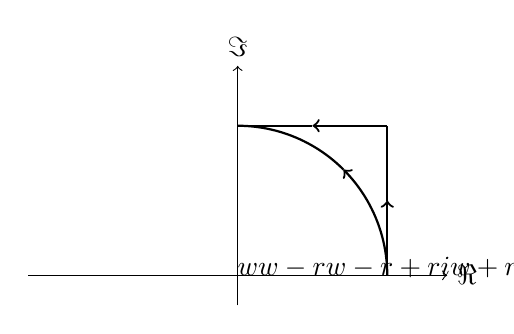
\begin{tikzpicture}[scale=1.9]
            % Axes
            \draw[->] (-1.4,0) -- (1.4,0) node[right] {$\Re$};
            \draw[->] (0,-0.2) -- (0,1.4) node[above] {$\Im$};
        
            % Quarter-circle contour
            \draw[thick, domain=0:45, ->] plot ({cos(\x)}, {sin(\x)});
            \draw[thick, domain=45:90, -] plot ({cos(\x)}, {sin(\x)});

            % Rectangular contour
            \draw[thick, ->] (1,0) -- (1,0.5);
            \draw[thick, -] (1,0.5) -- (1,1);
            \draw[thick, ->] (1,1) -- (0.5,1);
            \draw[thick, -] (0.5,1) -- (0,1);

            % Points of interest
            \labelledpoint{0}{0}{-0.3}{-0.8}{$w$}
            \labelledpoint{1}{0}{0}{-0.8}{$w - r$}
            \labelledpoint{1}{1}{0.3}{-0.2}{$w - r + ri$}
            \labelledpoint{0}{1}{-0.7}{-0.5}{$w + ri$}
        \end{tikzpicture}
        \caption{Contours for which \Cref{Ch4:Thm:CGTRectCircle} holds.}
    \end{subfigure} 
    \hfill
    \begin{subfigure}{0.48\linewidth}
        \centering
        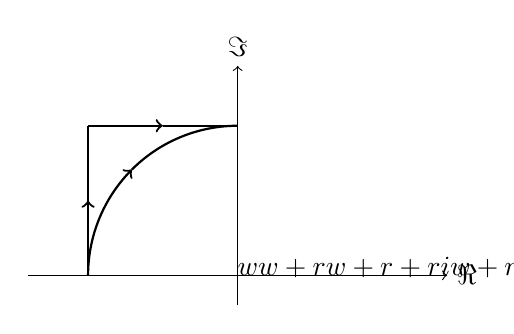
\begin{tikzpicture}[scale=1.9]
            % Axes
            \draw[->] (-1.4,0) -- (1.4,0) node[right] {$\Re$};
            \draw[->] (0,-0.2) -- (0,1.4) node[above] {$\Im$};
        
            % Quarter-circle contour
            \draw[thick, domain=180:135, ->] plot ({cos(\x)}, {sin(\x)});
            \draw[thick, domain=135:90, -] plot ({cos(\x)}, {sin(\x)});

            % Rectangular contour
            \draw[thick, ->] (-1,0) -- (-1,0.5);
            \draw[thick, -] (-1,0.5) -- (-1,1);
            \draw[thick, ->] (-1,1) -- (-0.5,1);
            \draw[thick, -] (-0.5,1) -- (0,1);

            % Points of interest
            \labelledpoint{0}{0}{0.3}{-0.8}{$w$}
            \labelledpoint{-1}{0}{0}{-0.8}{$w + r$}
            \labelledpoint{-1}{1}{-0.3}{-0.2}{$w + r + ri$}
            \labelledpoint{0}{1}{0.7}{-0.5}{$w + ri$}
        \end{tikzpicture}
        \caption{Contours for which an analogous result holds.}
        \label{Ch4:Subfig:CGTRectCircle_Alt}
    \end{subfigure} 
    \caption{The contour deformations permitted by \Cref{Ch4:Thm:CGTRectCircle}.}
\end{figure}

We now prove that $a$ is indeed a $+1$-eigenfunction of the Fourier transform.

\subsection{The $+1$-Eigenfunction}

The Fourier transform acts very interestingly on $a$. Recall from \Cref{Ch3:Thm:FourierSchwartz_CLE} that the Fourier transform is a linear isomorphism of Schwartz spaces. Since $I_1, \ldots, I_6$ are Schwartz, so are their compositions with the norm-squared function. Hence, for all $x \in \R^8$,
\begin{align*}
    \F\of{a(x)}
    % = \F\of{I_1\of{\norm{x}^2}} + \F\of{I_2\of{\norm{x}^2}} + \F\of{I_3\of{\norm{x}^2}} + \F\of{I_4\of{\norm{x}^2}} + \F\of{I_5\of{\norm{x}^2}} + \F\of{I_6\of{\norm{x}^2}}
    = \F\of{\sum_{j=1}^{6} I_j\of{\norm{x}^2}}
    = \sum_{j=1}^{6} \F\of{I_j\of{\norm{x}^2}}
\end{align*}

The strategy to show that $\F\of{a} = a$ will be to show that $\F$ acts on the $I_j\of{\norm{x}^2}$ in the following manner:\footnote{Note that we are abusing notation by denoting the function $x \mapsto I_j\of{\norm{x}^2} \in \Sch\of{\R^8, \C}$ by $I_j\of{\norm{x}^2}$.}
\begin{align}
    \F\of{I_1\of{\norm{x}^2} + I_2\of{\norm{x}^2}} &= I_3\of{\norm{x}^2} + I_4\of{\norm{x}^2} \label{Ch4:Eq:a_is_eig_perm_12_34} \\
    \F\of{I_3\of{\norm{x}^2} + I_4\of{\norm{x}^2}} &= I_1\of{\norm{x}^2} + I_2\of{\norm{x}^2} \label{Ch4:Eq:a_is_eig_perm_34_12} \\
    \F\of{I_5\of{\norm{x}^2}} &= I_6\of{\norm{x}^2} \label{Ch4:Eq:a_is_eig_perm_5_6} \\
    \F\of{I_6\of{\norm{x}^2}} &= I_5\of{\norm{x}^2} \label{Ch4:Eq:a_is_eig_perm_6_5}
\end{align}
Since, in addition to being Schwartz, all the $I_j\of{\norm{x}^2}$ (and their sums) are radial, \Cref{Ch3:Prop:RadialSchwartzFourier} tells us that \eqref{Ch4:Eq:a_is_eig_perm_34_12} and \eqref{Ch4:Eq:a_is_eig_perm_6_5} follow from \eqref{Ch4:Eq:a_is_eig_perm_12_34} and \eqref{Ch4:Eq:a_is_eig_perm_5_6} respectively. We now prove \eqref{Ch4:Eq:a_is_eig_perm_12_34} and \eqref{Ch4:Eq:a_is_eig_perm_5_6}.

As a preliminary step, though, we need to show integrability.

\begin{boxproposition}\label{Ch4:Prop:FourierIntegralConvergence_Ij}
    Fix $1 \leq j \leq 6$, and write $I_j(r) = \int_{X_j} f(r, z) \, \diff{z}$. Then, the Fourier Integral
    \begin{align*}
        \F\of{I_j\of{\norm{x}^2}}\of{\xi} = \int_{\R^8} \int_{X_j} \abs{f\of{\norm{x}^2, z} \, e^{-2 \pi i \cycl{x, \xi}}} \, \diff{z} \, \diff{x}
    \end{align*}
    converges for all $\xi \in \R^8$.
\end{boxproposition}
\begin{proof}
    Fix $\xi \in \R^8$. Note that we can disregard the $e^{-2 \pi i \cycl{x, \xi}}$ factor since it has absolute value $1$: the only reason we mention it is to emphasise that we are proving that the Fourier integral converges absolutely. Effectively, we need to show that the function
    \begin{align*}
        (x, z) \mapsto f\of{\norm{x}^2, z}
    \end{align*}
    admits an absolutely convergent integral over $\R^8 \times X_j$ with respect to the product measure.
    
    It has been formally verified that \href{https://github.com/leanprover-community/mathlib4/blob/5a2eaa85c555c4263e15928cef249cbaad2eb2d2/Mathlib/MeasureTheory/Integral/Prod.lean#L222-L238}{proving this is equivalent to proving the following two facts}.

    \begin{enumerate}
        \item \textbf{The integral over $X_j$ of the function $z \mapsto f\of{\norm{x}^2, z}$ is absolutely convergent for almost every $x \in \R^8$.}
        
        This is actually true for all $x$, and follows from the arguments in \Cref{Ch4:Subec:Schwartzness_a}.
        
        \item \textbf{The integral over $\R^8$ of the function $x 
        \mapsto \int_{X_j} \abs{f\of{\norm{x^2}, z}} \diff{z}$ is absolutely convergent.}
        
        By inspection, the arguments in \Cref{Ch4:Subec:Schwartzness_a} bound the function $r \mapsto \int_{X_j} \abs{f\of{r, z}} \diff{z}$ by a Schwartz function. Composing with the norm squared preserves Schwartzness by \Cref{Ch3:Prop:Multidimensional_Schwartz_of_Schwartz}, so we can bound the function $x \mapsto \int_{X_j} \abs{f\of{\norm{x}^2, z}} \diff{z}$ by a Schwartz function. It has been formally verified that \href{https://github.com/leanprover-community/mathlib4/blob/5a2eaa85c555c4263e15928cef249cbaad2eb2d2/Mathlib/Analysis/Distribution/SchwartzSpace.lean#L1095-L1097}{Schwartz functions are integrable}, so the integral over $\R^8$ of the function $x \mapsto \int_{X_j} \abs{f\of{\norm{x}^2, z}} \diff{z}$ must be absolutely convergent.
    \end{enumerate}
We can therefore conclude that the Fourier integral converges absolutely.
\end{proof}

Note that the above proposition is stronger than showing merely that the $I_j\of{\norm{x}^2}$ are integrable, as that does not imply that the integrands of the $I_j\of{\norm{x}^2}$ are integrable with respect to the product measure on $\R^8 \times X_j$. \Cref{Ch4:Prop:FourierIntegralConvergence_Ij}, however, does imply this, and we will need this to swap integrals using Fubini's theorem to prove the eigenfunction property.

\begin{boxlemma}\label{Ch4:Lemma:Fourier_I_1_add_I_2_eq_I_3_add_I_4}
    The Fourier transform % $\F : \Sch\of{\R^8, \C} \to \Sch{\R^8, \C}$
    maps $I_1\of{\norm{x}^2} + I_2\of{\norm{x}^2}$ to $I_3\of{\norm{x}^2} + I_4\of{\norm{x}^2}$.
\end{boxlemma}
\begin{proof}
    Since $\F$ acts linearly, we can treat $I_1$ and $I_2$ separately. For the purpose of this proof, denote the Fourier transforms of $I_1\of{\norm{x}^2}$ and $I_2\of{\norm{x}^2}$ by $F_1$ and $F_2$ respectively. Fix $\xi \in \R^8$. The integrability condition in \Cref{Ch4:Prop:FourierIntegralConvergence_Ij} allows us to change the order of integration below:
    \begin{align*}
        F_1\of{\xi} &= \int_{\R^8} \parenth {\int_{-1}^{-1 + i} \phi_0\of{\frac{-1}{z+1}} \, \parenth{z + 1}^2 \, e^{\pi i \norm{x}^2 z} \, \diff{z}} e^{-2\pi i \cycl{x, \xi}} \, \diff{x} \\
        &= \int_{-1}^{-1 + i} \phi_0\of{\frac{-1}{z+1}} \, \parenth{z + 1}^2 \parenth{\int_{\R^8} e^{\pi i \norm{x}^2 z} e^{-2\pi i \cycl{x, \xi} \diff{x}}} \, \diff{z}
    \end{align*}
    We can express $F_2$ in an analogous fashion. In both cases, the inner integral is exactly the Fourier integral of a Gaussian: in the notation of \Cref{Ch4:Thm:GaussianFourier}, $b = \pi i z$, and since $\Im(z) = \Re\of{i z} > 0$, we may apply the theorem to conclude that the inner integral is just
    \begin{align*}
        \frac{1}{z^4} \, e^{-\pi i \norm{\xi}^2 / z}
    \end{align*}
    We may therefore write
    \begin{align*}
        F_1\of{\xi} &= \int_{-1}^{-1 + i} \phi_0\of{\frac{-1}{z+1}} \, \parenth{z + 1}^2z^{-4} \, e^{\pi i \norm{\xi}^2 \parenth{\frac{-1}{z}}} \, \diff{z} \\
        F_2\of{\xi} &= \int_{-1 + i}^{i} \phi_0\of{\frac{-1}{z+1}} \, \parenth{z + 1}^2z^{-4} \, e^{\pi i \norm{\xi}^2 \parenth{\frac{-1}{z}}} \, \diff{z}
    \end{align*}
    We make a change of variables $w = \frac{-1}{z}$ in the above integrals. This Möbius transformation turns the vertical and horizontal contours in $F_1$ and $F_2$ into quarter-circular contours that we denote $\gamma_1$ and $\gamma_2$ respectively. See \Cref{Ch4:Fig:Eigenfunction_Mobius_Contours}.

    \begin{figure}[htb]
        \centering
        \begin{subfigure}{0.4\linewidth}
            \centering
            \begin{tikzpicture}[scale=1.9]
                % Axes
                \draw[->] (-1.4,0) -- (1.4,0) node[right] {$\Re$};
                \draw[->] (0,-0.2) -- (0,1.4) node[above] {$\Im$};
    
                % F_1
                \draw[thick, ->] (-1,0) -- (-1,0.5);
                \draw[thick, -] (-1,0.5) -- (-1,1);

                % F_2
                \draw[thick, ->] (-1,1) -- (-0.5,1);
                \draw[thick, -] (-0.5,1) -- (0,1);
    
                % Points of interest
                % \labelledpoint{0}{0}{0.3}{-0.8}{$0$}
                \labelledpoint{-1}{0}{0}{-0.8}{$-1$}
                \labelledpoint{-1}{1}{-0.3}{-0.2}{$-1 + i$}
                \labelledpoint{0}{1}{0.3}{-0.4}{$i$}
            \end{tikzpicture}
            \caption{Before the transformation}
        \end{subfigure}
        \begin{subfigure}{0.1\linewidth}
            \vfill
            \[ \leadsto \]
            \vspace{5em}
        \end{subfigure}
        \begin{subfigure}{0.4\linewidth}
            \centering
            \begin{tikzpicture}[scale=1.9]
                % Axes
                \draw[->] (-1.4,0) -- (1.4,0) node[right] {$\Re$};
                \draw[->] (0,-0.2) -- (0,1.4) node[above] {$\Im$};
            
                % \gamma_1
                \draw[thick, domain=0:45, ->] plot ({0.5 + 0.5 * cos(\x)}, {0.5 * sin(\x)}) node[below left] {$\gamma_1$};
                \draw[thick, domain=45:90, -] plot ({0.5 + 0.5 * cos(\x)}, {0.5 * sin(\x)});

                % \gamma_2
                \draw[thick, domain=0:45, ->] plot ({0.5 * cos(\x)}, {0.5 + 0.5 * sin(\x)}) node[below left] {$\gamma_2$};
                \draw[thick, domain=45:90, -] plot ({0.5 * cos(\x)}, {0.5 + 0.5 * sin(\x)});
    
                % Points of interest
                % \labelledpoint{0}{0}{0.3}{-0.8}{$w$}
                \labelledpoint{1}{0}{0}{-0.8}{$1$}
                \labelledpoint{0.5}{0.5}{0.6}{-0.2}{$\frac{1}{2} + \frac{1}{2}i$}
                \labelledpoint{0}{1}{-0.3}{-0.4}{$i$}
            \end{tikzpicture}
            \caption{After the transformation}
        \end{subfigure}
        \caption{The effect of the Möbius transformation $z \mapsto -1/z$ on the contours of $F_1$ and $F_2$}
        \label{Ch4:Fig:Eigenfunction_Mobius_Contours}
    \end{figure}
    Treating $\xi$ as a constant and denoting
    \begin{align*}
        f(w) := \phi_0\of{-1 - \frac{1}{w - 1}} \, \parenth{\frac{-1}{w} + 1}^2 w^2 \, e^{\pi i \norm{\xi}^2 w}
    \end{align*}
    we can distribute the $w^2$ term and use the fact that $\phi_0$ is $1$-periodic (cf. \eqref{Ch4:Eq:phi_0_add_one}) to write
    \begin{align*}
        f(w) = \phi_0\of{\frac{-1}{w - 1}} \, \parenth{w - 1}^2 \, e^{\pi i \norm{\xi}^2 w}
    \end{align*}
    we note that $f$ is holomorphic (in $w$) on the upper half-plane. \Cref{Ch4:Thm:CGTRectCircle} then tells us the following.
    \begin{align*}
        F_1\of{\xi}
        &= \int_{\gamma_1} f(w) \, \diff{w}
        = \int_{1}^{1 + \frac{1}{2}i} f(w) \, \diff{w}
        + \int_{1 + \frac{i}{2}i}^{\frac{1}{2} + \frac{1}{2}i} f(w) \, \diff{w} \\
        F_2\of{\xi}
        &= \int_{\gamma_2} f(w) \, \diff{w}
        = \int_{\frac{1}{2} + \frac{1}{2}i}^{\frac{1}{2} + i} f(w) \, \diff{w}
        + \int_{\frac{1}{2} + i}^{i} f(w) \, \diff{w}
    \end{align*}
    The \CGT\ for rectangles, which has been \href{https://github.com/leanprover-community/mathlib4/blob/88928cefd7edb1ba61623bffd4e86389dfe1f648/Mathlib/Analysis/Complex/CauchyIntegral.lean#L245}{formally verified}, tells us that
    \begin{align*}
        \int_{1 + \frac{i}{2}i}^{\frac{1}{2} + \frac{1}{2}i} f(w) \, \diff{w}
        + \int_{\frac{1}{2} + \frac{1}{2}i}^{\frac{1}{2} + i} f(w) \, \diff{w}
        = \int_{1 + \frac{1}{2}i}^{1+i} f(w) \, \diff{w}
        + \int_{1+i}^{\frac{1}{2} + i} f(w) \, \diff{w}
    \end{align*}
    Therefore, we can express $F_1 + F_2$ in the following manner:
    \begin{align*}
        F_1\of{\xi} + F_2\of{\xi}
        &= \int_{1}^{1 + \frac{1}{2}i} f(w) \, \diff{w}
        + \parenth{\int_{1 + \frac{i}{2}i}^{\frac{1}{2} + \frac{1}{2}i} f(w) \, \diff{w}
        + \int_{\frac{1}{2} + \frac{1}{2}i}^{\frac{1}{2} + i} f(w) \, \diff{w}}
        + \int_{\frac{1}{2} + i}^{i} f(w) \, \diff{w} \\
        &= \parenth{\int_{1}^{1 + \frac{1}{2}i} f(w) \, \diff{w}
        + \int_{1 + \frac{1}{2}i}^{1+i} f(w) \, \diff{w}}
        + \parenth{\int_{1+i}^{\frac{1}{2} + i} f(w) \, \diff{w}
        + \int_{\frac{1}{2} + i}^{i} f(w) \, \diff{w}} \\
        &= I_3\of{\norm{\xi}^2} + I_4\of{\norm{\xi}^2}
    \end{align*}
    as required. \Cref{Ch4:Fig:Eigenfunction_CauchyGoursat_a} shows how contours were modified over the course of this argument.
    \begin{figure}[hbt]
        \centering
        \begin{subfigure}{0.4\linewidth}
            \centering
            \begin{tikzpicture}[scale=1.9]
                % Axes
                \draw[->] (-1.4,0) -- (1.4,0) node[right] {$\Re$};
                \draw[->] (0,-0.2) -- (0,1.4) node[above] {$\Im$};
            
                % \gamma_1
                \draw[thick, domain=0:45, ->, red] plot ({0.5 + 0.5 * cos(\x)}, {0.5 * sin(\x)}) node[below left] {$\gamma_1$};
                \draw[thick, domain=45:90, -, red] plot ({0.5 + 0.5 * cos(\x)}, {0.5 * sin(\x)});

                % \gamma_2
                \draw[thick, domain=0:45, ->, red] plot ({0.5 * cos(\x)}, {0.5 + 0.5 * sin(\x)}) node[below left] {$\gamma_2$};
                \draw[thick, domain=45:90, -, red] plot ({0.5 * cos(\x)}, {0.5 + 0.5 * sin(\x)});

                % Rectangle 1
                \draw[thick, ->, darkgreen] (1, 0) -- (1, 0.25);
                \draw[thick, -, darkgreen] (1, 0.25) -- (1, 0.5);
                \draw[thick, ->, darkgreen] (1, 0.5) -- (0.75, 0.5);
                \draw[thick, -, darkgreen] (0.75, 0.5) -- (0.5, 0.5);

                % Rectangle 2
                \draw[thick, ->, darkgreen] (0.5, 0.5) -- (0.5, 0.75);
                \draw[thick, -, darkgreen] (0.5, 0.75) -- (0.5, 1);
                \draw[thick, ->, darkgreen] (0.5, 1) -- (0.25, 1);
                \draw[thick, -, darkgreen] (0.25, 1) -- (0, 1);
    
                % Points of interest
                % \labelledpoint{0}{0}{0.3}{-0.8}{$w$}
                \labelledpoint{1}{0}{0}{-0.8}{$1$}
                \labelledpoint{0.5}{0.5}{0.6}{-0.2}{}
                \labelledpoint{0}{1}{-0.3}{-0.4}{$i$}
            \end{tikzpicture}
            \caption{Changing contours from circles to rectangles}
        \end{subfigure}
        \hfill
        \begin{subfigure}{0.4\linewidth}
            \centering
            \begin{tikzpicture}[scale=1.9]
                % Axes
                \draw[->] (-1.4,0) -- (1.4,0) node[right] {$\Re$};
                \draw[->] (0,-0.2) -- (0,1.4) node[above] {$\Im$};
            
                % Rectangle 1
                \draw[thick, ->] (1, 0) -- (1, 0.25);
                \draw[thick, -] (1, 0.25) -- (1, 0.5);
                \draw[thick, ->, red] (1, 0.5) -- (0.75, 0.5);
                \draw[thick, -, red] (0.75, 0.5) -- (0.5, 0.5);

                % Rectangle 2
                \draw[thick, ->, red] (0.5, 0.5) -- (0.5, 0.75);
                \draw[thick, -, red] (0.5, 0.75) -- (0.5, 1);
                \draw[thick, ->] (0.5, 1) -- (0.25, 1);
                \draw[thick, -] (0.25, 1) -- (0, 1);

                % Rectangle Cauchy-Goursat
                \draw[thick, ->, darkgreen] (1, 0.5) -- (1, 0.75);
                \draw[thick, -, darkgreen] (1, 0.5) -- (1, 1);
                \draw[thick, ->, darkgreen] (1, 1) -- (0.75, 1);
                \draw[thick, -, darkgreen] (0.75, 1) -- (0.5, 1);
    
                % Points of interest
                % \labelledpoint{0}{0}{0.3}{-0.8}{$w$}
                \labelledpoint{1}{0}{0}{-0.8}{$1$}
                \labelledpoint{0.5}{0.5}{0.6}{-0.2}{}
                \labelledpoint{0}{1}{-0.3}{-0.4}{$i$}
            \end{tikzpicture}
            \caption{Changing rectangular contours to get $I_3$ and $I_4$}
        \end{subfigure}
        \caption{Applying the two versions of the \CGT\ to prove the result. In the proof, contours were changed from red to green.}
        \label{Ch4:Fig:Eigenfunction_CauchyGoursat_a}
    \end{figure}
\end{proof}

The proof that the Fourier transform maps $I_5$ to $I_6$ is nearly identical in structure but significantly simpler, because the Möbius transformation $z \mapsto \frac{-1}{z}$ simply maps the contour in $I_5$ to that in $I_6$ (and vice-versa). We omit the proof.

In summary, we have shown that the Fourier transform permutes the integrals that make up $a$, thereby not changing $a$. $a$ is thus an eigenfunction of $\F$ with eigenvalue $1$.

It is worth noting that the Möbius transformation $z \mapsto \frac{-1}{z}$ in the proof of \Cref{Ch4:Lemma:Fourier_I_1_add_I_2_eq_I_3_add_I_4} has derivative $\frac{1}{z^2}$, which reduces the $z^4$ term in the integrand to $z^2$, which matches the pattern in $I_3$ and $I_4$. However, the reason the $z^4$ term arises is that we take the $8$-dimensional Fourier transform of an $8$-dimensional Gaussian. This illustrates why it was necessary to treat $a$ as an $\R^8 \to \C$ function to show the eigenfunction property. More generally, despite Fourier transforms being linear isomorphisms of Schwartz spaces, the fact remains that in different Schwartz spaces, the Fourier transform operators may be fundamentally different, and linear maps between Schwartz spaces are not guaranteed to preserve the Fourier transform operator.

We now use similar techniques to show that $b$ is a Fourier eigenfunction with eigenvalue $-1$. % Just as we did with the proof of Schwartzness, we omit repetitive arguments and focus on the key distinctions between the two cases.

\subsection{The $-1$-Eigenfunction}
\section{Establishing the Double Zeroes Property}

% At some point earlier on, maybe in Chapter 3, we need to stress that double zeroes means double zeroes in the radial sense, except double zeroes after composition with just the norm and not the norm squared. (We are using norm squared so that we can prove Schwartzness. Just the norm isn't enough because the norm isn't smooth.)

The way we prove that $a$ and $b$ have double zeroes at $E_8$ lattice points with norm $> \sqrt{2}$ (or at normalised $E_8$ lattice points with norm $> 1$) is by showing that $a\rad$ and $b\rad$ agree, for $r > 2$, with functions that have double zeroes at \textit{all} even integers. It will then follow that $a$ and $b$ have double zeroes at all points on the $E_8$ lattice with norm $> \sqrt{2}$, since all elements of $\Lambda_8$ have norm of the form $\sqrt{2n}$ for some $n \in \N$ (cf. \sorry).\todo{ADD RESULT TO E8 SECTION}

The strategy to prove these two equalities will be to perform a change of contours using a version of the Cauchy-Goursat Theorem and use the relations and transformation rules between the $\phi$- and $\psi$-functions to combine integrals so that the result is exactly $a\rad$ or $b\rad$.

The version of the Cauchy-Goursat Theorem we use is the following.

\begin{boxtheorem}[Cauchy-Goursat for Unbounded Contours]\label{Ch4:Thm:CauchyGoursat_Unbounded}
    Suppose $f : \C \to \C$ is a function such that $f(z) \to 0$ as $\Im(z) \to \infty$. Then, for all $x_1, y_1, x_2, y_2 \in \R$, if $f$ is holomorphic at $z$ for all $z \in \C$ with $x_1 < \Re(z) < x_2$ and $y_2 < \Im(z)$, then
    \begin{align*}
        \int_{x_1 + iy_1}^{x_1 + i\infty} f(z) \, \diff{z}
        = \int_{x_1 + iy_1}^{x_1 + iy_2} f(z) \, \diff{z}
        + \int_{x_1 + iy_2}^{x_2 + iy_2} f(z) \, \diff{z}
        + \int_{x_2 + iy_2}^{x_2 + i\infty} f(z) \, \diff{z}
    \end{align*}
    provided that $f$ is integrable on the unbounded vertical contours.
\end{boxtheorem}

\begin{wrapfigure}[7]{r}{0.4\linewidth}
    \vspace{-0.7em}
    \centering
    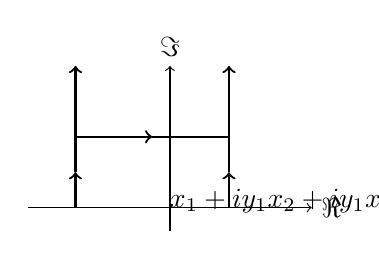
\begin{tikzpicture}[scale=1.5]
        % Axes
        \draw[->] (-1.2,0) -- (1.2,0) node[right] {$\Re$};
        \draw[->] (0,-0.2) -- (0,1.2) node[above] {$\Im$};
    
        % Contours
        \draw[thick, ->] (-0.8, 0) -- (-0.8,0.3);
        \draw[thick, ->] (-0.8,0.3) -- (-0.8, 1.2);
        \draw[thick, ->] (0.5, 0) -- (0.5,0.3);
        \draw[thick, ->] (0.5,0.3) -- (0.5, 1.2);
        \draw[thick, ->] (-0.8, 0.6) -- (-0.15, 0.6);
        \draw[thick] (-0.15, 0.6) -- (0.5, 0.6);
    
        % Points of interest
        \labelledpoint{-0.8}{0}{-0.4}{-0.8}{$x_1 + iy_1$}
        \labelledpoint{0.5}{0}{0.4}{-0.8}{$x_2 + iy_1$}
        \labelledpoint{-0.8}{0.6}{-0.8}{-0.3}{$x_1 + iy_2$}
        \labelledpoint{0.5}{0.6}{0.8}{-0.3}{$x_2 + iy_2$}
    \end{tikzpicture}
    \caption{Visualising the contours in \Cref{Ch4:Thm:CauchyGoursat_Unbounded}.}  
\end{wrapfigure}

We discuss the informal and formal proofs of this theorem in \Cref{Ch5:Sec:Cauchy-Goursat}.

For both $a\rad$ and $b\rad$, we begin by their alternate expressions for them. We then make estimates to prove that the integrals in these expressions converge. We finally manipulate the expressions and apply \Cref{Ch4:Thm:CauchyGoursat_Unbounded} to show that they do, indeed, agree with $a\rad$ and $b\rad$ on inputs $> 2$.

\subsection{The $+1$-Eigenfunction}

We begin by defining the integral by which we represent $a\rad$.

\begin{boxdefinition}[Alternate Representation of $a$]
    Define $d : \parenth{2, \infty} \to \C$ by
    \begin{align*}
        d\of{r} = -4 \sinsq{\frac{\pi r}{2}} \int_{0}^{i\infty} \phi_0\of{\frac{-1}{z}} \, z^2 \, e^{\pi i r z} \, \diff{z}
    \end{align*}
    for all $r \in \parenth{2, \infty}$.
\end{boxdefinition}

It is clear that we can parametrise the integral in $d$ by $z = it$ for $t \in \parenth{0, \infty}$, and write
\begin{align}
    d(r) = 4i \sinsq{\frac{\pi r}{2}} \int_{0}^{\infty} \phi_0\of{\frac{i}{t}} \, t^2 \, e^{-\pi r t} \, \diff{t}
    \label{Ch4:Eq:d_parametrised}
\end{align}

We begin by showing that this integral converges for $r > 2$. We do this by estimating the integrand.

\begin{boxlemma}
    $\exists C_0 > 0$ such that for $t \in \parenth{0, 2}$, $\abs{\phi_0\of{\frac{i}{t}}} \leq C_0 \, e^{-2\pi/t}$.
\end{boxlemma}
\begin{proof}
    The result then follows immediately from \eqref{Ch4:Eq:PolyFourierCoeffBound_phi_0}, with $z = i/t$.
\end{proof}

We can hence conclude that for $t \in \parenth{0, 2}$, the integrand in \eqref{Ch4:Eq:d_parametrised} is bounded:
\begin{align*}
    \abs{\phi_0\of{\frac{i}{t}} \, t^2 \, e^{-\pi r t}} 
    \leq 4 C_0 \, e^{-2\pi / t} \, e^{-\pi r t}
    \leq 4 C_0
\end{align*}

We can also estimate the integrand for $t \geq 2$.

\begin{boxlemma}\label{Ch4:Lemma:d_integral_estimate_above}
    $\exists C > 0$ such that for $t \geq 2$, $\abs{\phi_{0}\of{\frac{i}{t}}} \leq C t^{-2} e^{2\pi t}$.
\end{boxlemma}
\begin{proof}
    From \eqref{Ch4:Eq:phi_0_neg_inv}, we know that for all $t \geq 2$,
    \begin{align*}
        \abs{\phi_0\of{\frac{i}{t}}}
        = \abs{\phi_{0}\of{\frac{-1}{it}}}
        \leq \abs{\phi_{0\of{it}}} + \frac{12}{\pi t} \abs{\phi_{-2}\of{it}} + \frac{36}{\pi^2 t^2} \abs{\phi_{-4}\of{it}}
    \end{align*}
    Estimating each of these terms using \Cref{Ch4:Lemma:PolyFourierCoeffBound_Apply_a}, we know $\exists C_0, C_{-2}, C_{-4} > 0$ such that
    \begin{align*}
        \abs{\phi_{0}\of{it}} + \frac{12}{\pi t} \abs{\phi_{-2}\of{it}} + \frac{36}{\pi^2 t^2} \abs{\phi_{-4}\of{it}}
        \leq C_0 e^{-2 \pi t} + \frac{12}{\pi t} C_{-2} + \frac{36}{\pi^2 t^2} C_{-4} e^{2 \pi t}
    \end{align*}
    For $t \geq 2$, $C_0 e^{-2 \pi t}$ and $\frac{12}{\pi t} C_{-2}$ are clearly bounded by constants, and the growth of the above expression is dominated by $t^{-2} e^{2\pi t}$. Hence, we can conclude that $\exists C > 0$ such that for $t \geq 2$, $\abs{\phi_0\of{\frac{i}{t}}} \leq C t^{-2} e^{2 \pi t}$, as required.
\end{proof}

We can hence conclude that for $t \geq 2$, the integrand in \eqref{Ch4:Eq:d_parametrised} is bounded by an integrable function:
\begin{align*}
    \abs{\phi_0\of{\frac{i}{t}} \, t^2 \, e^{-\pi r t}} 
    \leq C \parenth{t^{-2} e^{2\pi t}} \parenth{t^2 e^{-\pi r t}}
    = C e^{\pi t \parenth{2 - r}}
\end{align*}
Here, we require $r > 2$ so that the exponent is negative. Since $d$ was defined precisely on such $r$, we can conclude that the integral in the definition of $d$ converges absolutely.

Arguing as above yields another important result.
\begin{boxlemma}
    For all $r > 2$ and $z \in \Halfplane$, as $\Im(z) \to \infty$,
    \begin{align*}
        \phi_{0}\of{\frac{-1}{z}} \, z^2 \, e^{\pi i r z} \to 0
    \end{align*}
\end{boxlemma}
\begin{proof}[Proof sketch]
    We do not offer more than a sketch here because the proof is almost identical to that of \Cref{Ch4:Lemma:d_integral_estimate_above}. The idea is to apply \eqref{Ch4:Eq:phi_0_neg_inv}, multiply through, apply \Cref{Ch4:Lemma:PolyFourierCoeffBound_Apply_a} to bound the expression in absolute value, and use the fact that $r > 2$ to conclude that the bound decays exponentially as $\Im(z) \to \infty$.
\end{proof}

The function $z \mapsto \phi_{0}\of{\frac{-1}{z}} \, z^2 \, e^{\pi i r z}$ is also holomorphic on $\Halfplane$, a fact that is again seen by applying \eqref{Ch4:Eq:phi_0_neg_inv} and the fact that the numerators of the $\phi$-function are holomorphic and the denominators are non-vanishing on $\Halfplane$.

We are now ready to show the following.

\begin{boxproposition}
    For all $r > 2$, $d(r) = a\rad(r)$.
\end{boxproposition}
\begin{proof}
    Fix $r > 2$. We begin by performing the following manipulation:
    \begin{align*}
        -4 \sinsq{\frac{\pi r}{2}}
        = -4 \parenth{\frac{e^{i \pi r / 2} - e^{-i \pi r / 2}}{2i}}^2
        = \parenth{e^{i \pi r / 2} - e^{- i \pi r / 2}}^2
        = e^{i \pi r} - 2 + e^{-i \pi r}
    \end{align*}
    Therefore, for all $r > 2$,
    \begin{align*}
        d(r)
        &= -4 \sinsq{\frac{\pi r}{2}} \int_{0}^{i \infty} \phi_0\of{\frac{-1}{z}} \, z^2 \, e^{\pi i r z} \, \diff{z}
        = \parenth{e^{i \pi r} - 2 + e^{-i \pi r}} \int_{0}^{i \infty} \phi_0\of{\frac{-1}{z}} \, z^2 \, e^{\pi i r z} \, \diff{z} \\
        &= \int_{0}^{i \infty} \phi_0\of{\frac{-1}{z}} z^2 \, e^{\pi i r \parenth{z + 1}} \, \diff{z}
        -2 \int_{0}^{i \infty} \phi_0\of{\frac{-1}{z}} z^2 \, e^{\pi i r z} \, \diff{z}
        + \int_{0}^{i \infty} \phi_0\of{\frac{-1}{z}} z^2 \, e^{\pi i r \parenth{z - 1}} \, \diff{z}
    \end{align*}
    By a simple change of variables, we can rewrite the first and third integrals as follows. We can also split the second integral into two parts as shown below.
    \begin{align*}
        \int_{0}^{i \infty} \phi_0\of{\frac{-1}{z}} z^2 \, e^{\pi i r \parenth{z - 1}} \, \diff{z}
        &=
        \int_{-1}^{-1 + i \infty} \phi_0\of{\frac{-1}{z + 1}} \parenth{z + 1}^2 \, e^{\pi i r z} \, \diff{z} \\
        \int_{0}^{i \infty} \phi_0\of{\frac{-1}{z}} z^2 \, e^{\pi i r \parenth{z + 1}} \, \diff{z}
        &=
        \int_{1}^{1 + i \infty} \phi_0\of{\frac{-1}{z - 1}} \parenth{z - 1}^2 \, e^{\pi i r z} \, \diff{z} \\
        -2 \int_{0}^{i \infty} \phi_0\of{\frac{-1}{z}} z^2 \, e^{\pi i r z} \, \diff{z}
        &=
        -2 \int_{0}^{i} \phi_0\of{\frac{-1}{z}} z^2 \, e^{\pi i r z} \, \diff{z}
        -2 \int_{i}^{i \infty} \phi_0\of{\frac{-1}{z}} z^2 \, e^{\pi i r z} \, \diff{z} \\
        &= I_5(r) - 2\int_{i}^{i \infty} \phi_0\of{\frac{-1}{z}} z^2 \, e^{\pi i r z} \, \diff{z}
    \end{align*}
    We can now apply \Cref{Ch4:Thm:CauchyGoursat_Unbounded} to the first and third integrals, noting that the required integrability conditions do hold because the integrals making up $d$ and $a\rad$ converge absolutely.
    \begin{align*}
        \int_{-1}^{-1 + i \infty} \phi_0\of{\frac{-1}{z + 1}} \parenth{z + 1}^2 \, e^{\pi i r z} \, \diff{z}
        =& \int_{-1}^{-1 + i} \phi_0\of{\frac{-1}{z + 1}} \parenth{z + 1}^2 \, e^{\pi i r z} \, \diff{z} \\
        &+ \int_{-1 + i}^{i} \phi_0\of{\frac{-1}{z + 1}} \parenth{z + 1}^2 \, e^{\pi i r z} \, \diff{z} \\
        &+ \int_{i}^{i \infty} \phi_0\of{\frac{-1}{z + 1}} \parenth{z + 1}^2 \, e^{\pi i r z} \, \diff{z} \\
        =& I_1(r) + I_2(r) + \int_{i}^{i \infty} \phi_0\of{\frac{-1}{z + 1}} \parenth{z + 1}^2 \, e^{\pi i r z} \, \diff{z} \\
        \int_{1}^{1 + i \infty} \phi_0\of{\frac{-1}{z - 1}} \parenth{z - 1}^2 \, e^{\pi i r z} \, \diff{z}
        =& \int_{1}^{1 + i} \phi_0\of{\frac{-1}{z - 1}} \parenth{z - 1}^2 \, e^{\pi i r z} \, \diff{z} \\
        &+ \int_{1 + i}^{i} \phi_0\of{\frac{-1}{z - 1}} \parenth{z - 1}^2 \, e^{\pi i r z} \, \diff{z} \\
        &+ \int_{i}^{i \infty} \phi_0\of{\frac{-1}{z - 1}} \parenth{z - 1}^2 \, e^{\pi i r z} \, \diff{z} \\
        =& I_3(r) + I_4(r) + \int_{i}^{i \infty} \phi_0\of{\frac{-1}{z - 1}} \parenth{z - 1}^2 \, e^{\pi i r z} \, \diff{z}
    \end{align*}
    Hence, we can express $d(r)$ as the sum of the following six integrals:
    \begin{align*}
        d(r) =& I_1(r) + I_2(r) + I_3(r) + I_4(r) + I_5(r) \\
        &+ \int_{i}^{i\infty} \parenth{
            \phi_0\of{\frac{-1}{z + 1}} \parenth{z + 1}^2 \, e^{\pi i r z} +
            \phi_0\of{\frac{-1}{z - 1}} \parenth{z - 1}^2 \, e^{\pi i r z} - 2
            \phi_0\of{\frac{-1}{z}} z^2 \, e^{\pi i r z}
        } \, \diff{z}
    \end{align*}
    One can show, by applying \eqref{Ch4:Eq:phi_0_neg_inv} and simplifying, that
    \begin{align*}
        \phi_0\of{\frac{-1}{z + 1}} \parenth{z + 1}^2 +
        \phi_0\of{\frac{-1}{z - 1}} \parenth{z - 1}^2 +
        \phi_0\of{\frac{-1}{z}} z^2 = 2\phi_0
    \end{align*}
    Hence, the sixth integral above is precisely $I_6$, proving that $d(r) = a\rad(r)$ for all $r > 2$.
\end{proof}

The factor of $-4\sinsq{\pi r / 2}$ in the definition of $d$ then ensures that $a\rad$ has double zeroes at all even integers except possibly $0$ and $\pm 2$, which allows us to conclude that $a$ has double zeroes at all points in $\R^8$---particularly those lying on $\Lambda_8$---with norm of the form $\sqrt{2n}$ for $n \in \N \setminus \set{0, 1}$.

\subsection{The $-1$-Eigenfunction}
\section{The Magic of $g$}
\label{Ch4:Sec:g_Properties}

% Not yet sure how this section should look